\documentclass[a4paper,12pt,times,print,index,custombib,custommargin]{PhDThesisPSnPDF}\usepackage[]{graphicx}\usepackage[]{color}
%% maxwidth is the original width if it is less than linewidth
%% otherwise use linewidth (to make sure the graphics do not exceed the margin)
\makeatletter
\def\maxwidth{ %
  \ifdim\Gin@nat@width>\linewidth
    \linewidth
  \else
    \Gin@nat@width
  \fi
}
\makeatother

\definecolor{fgcolor}{rgb}{0.345, 0.345, 0.345}
\newcommand{\hlnum}[1]{\textcolor[rgb]{0.686,0.059,0.569}{#1}}%
\newcommand{\hlstr}[1]{\textcolor[rgb]{0.192,0.494,0.8}{#1}}%
\newcommand{\hlcom}[1]{\textcolor[rgb]{0.678,0.584,0.686}{\textit{#1}}}%
\newcommand{\hlopt}[1]{\textcolor[rgb]{0,0,0}{#1}}%
\newcommand{\hlstd}[1]{\textcolor[rgb]{0.345,0.345,0.345}{#1}}%
\newcommand{\hlkwa}[1]{\textcolor[rgb]{0.161,0.373,0.58}{\textbf{#1}}}%
\newcommand{\hlkwb}[1]{\textcolor[rgb]{0.69,0.353,0.396}{#1}}%
\newcommand{\hlkwc}[1]{\textcolor[rgb]{0.333,0.667,0.333}{#1}}%
\newcommand{\hlkwd}[1]{\textcolor[rgb]{0.737,0.353,0.396}{\textbf{#1}}}%

\usepackage{framed}
\makeatletter
\newenvironment{kframe}{%
 \def\at@end@of@kframe{}%
 \ifinner\ifhmode%
  \def\at@end@of@kframe{\end{minipage}}%
  \begin{minipage}{\columnwidth}%
 \fi\fi%
 \def\FrameCommand##1{\hskip\@totalleftmargin \hskip-\fboxsep
 \colorbox{shadecolor}{##1}\hskip-\fboxsep
     % There is no \\@totalrightmargin, so:
     \hskip-\linewidth \hskip-\@totalleftmargin \hskip\columnwidth}%
 \MakeFramed {\advance\hsize-\width
   \@totalleftmargin\z@ \linewidth\hsize
   \@setminipage}}%
 {\par\unskip\endMakeFramed%
 \at@end@of@kframe}
\makeatother

\definecolor{shadecolor}{rgb}{.97, .97, .97}
\definecolor{messagecolor}{rgb}{0, 0, 0}
\definecolor{warningcolor}{rgb}{1, 0, 1}
\definecolor{errorcolor}{rgb}{1, 0, 0}
\newenvironment{knitrout}{}{} % an empty environment to be redefined in TeX

\usepackage{alltt}
%\documentclass[a4paper,12pt,times,numbered,print,index]{PhDThesisPSnPDF}

\usepackage{import}

% ******************************************************************************
% ****************************** Custom Margin *********************************

% Add `custommargin' in the document class options to use this section
% Set {innerside margin / outerside margin / topmargin / bottom margin}  and
% other page dimensions
\ifsetCustomMargin
  \RequirePackage[left=42mm,right=35mm,top=25mm,bottom=20mm]{geometry}
  \setFancyHdr % To apply fancy header after geometry package is loaded
\fi

% *****************************************************************************
% ******************* Fonts (like different typewriter fonts etc.)*************

% Add `customfont' in the document class option to use this section

\ifsetCustomFont
  % Set your custom font here and use `customfont' in options. Leave empty to
  % load computer modern font (default LaTeX font).
  \RequirePackage{helvet}
\fi

% *****************************************************************************
% **************************** Custom Packages ********************************
\usepackage{import}

%\usepackage{comment}

\usepackage{epigraph}

%% ---- package for formatting code with line numbers
\usepackage{fancyvrb} %% for verbatim text

\usepackage{ulem} % more underlining and other font effects

% ************************** Custom Floats **********************************
\usepackage{float}
\floatstyle{ruled}
\newfloat{cmd}{htb}{loc}[chapter]
\floatname{cmd}{Command}
% **** **** **** **** **** **** **** ****

%% ---- provides "\rowcolors" command
\usepackage[dvipsnames,table]{xcolor}

\usepackage{subcaption}

% ---- the following package call ensures that floats will not pass a section boundary ----
\usepackage[section]{placeins}
% ---- insert “\FloatBarrier” at places that floats should not move past, perhaps at every “\section”.

% ---- if I want to extract LaTeX formulas, for instance, 
% ---- to convert them into other picture formats from pdf
%\usepackage[active,tightpage]{preview}
% ---- use \begin{preiview} ... \end{preview}

\usepackage{relsize}
\renewcommand\RSsmallest{4pt}

%------ the following package can be used for Word Review function mimicking comments ----------%
\usepackage[textsize=tiny, textwidth=3cm, color=Dandelion, colorinlistoftodos]{todonotes} % specify ``disable'' to turn off all notes
\newcommand{\addcit}[1]{\todo[color=yellow!90,nolist]{#1}}
\newcommand{\comment}[1]{\todo[color=green!40,noline,nolist]{#1}} % the "comment" package also defines a command "\comment", so cannot use both
\newcommand{\longcomment}[1]{\todo[color=green!40,inline,nolist]{#1}}
\newcommand{\roger}[1]{\todo[color=blue!40]{Roger:\newline{}#1}}

%\ifsetDraft
%	\usepackage[textsize=tiny, textwidth=3cm, color=Dandelion, colorinlistoftodos]{todonotes} % specify ``disable'' to turn off all notes
%	\newcommand{\addcit}[1]{\todo[color=yellow!90,nolist]{#1}}
%	\newcommand{\comment}[1]{\todo[color=green!40,noline,nolist]{#1}}
%	\newcommand{\longcomment}[1]{\todo[color=green!40,inline,nolist]{#1}}
%	\newcommand{\roger}[1]{\todo[color=blue!40]{Roger:\newline{}#1}}
%\else
%	\newcommand{\addcit}[1]{}
%	\newcommand{\comment}[1]{}
%	\newcommand{\longcomment}[1]{}
%	\newcommand{\roger}[1]{}
%	\newcommand{\listoftodos}{}
%	\newcommand{\todo}{}
%\fi

%\usepackage{setspace}
%\newcommand{\note}[2][] {\todo[caption={#2}, #1] {\begin{spacing}{0.8}#2\end{spacing}}}

\usepackage{pdflscape}
\usepackage{lscape} % offers landscape environment, \begin{landscape}

% ---- for verbatim in captions. Usage: \cprotect\caption{...} ----
\usepackage{cprotect} 


% ************************* Algorithms and Pseudocode **************************

%\usepackage{algpseudocode}


% ********************Captions and Hyperreferencing / URL **********************

% Captions: This makes captions of figures use a boldfaced small font.
%\RequirePackage[small,bf]{caption}

\RequirePackage[labelsep=space,font=small,labelfont=bf,tableposition=top]{caption}
\DeclareCaptionLabelFormat{continued}{#1 #2 continued} 
\captionsetup[ContinuedFloat]{labelformat=continued}
\renewcommand{\figurename}{Fig.} %to support older versions of captions.sty
\usepackage{varioref}

\hypersetup{%
colorlinks=true,% 
citecolor=black,% 
linkcolor=black,
urlcolor=black% 
}



% *************************** Graphics and figures *****************************

%\usepackage{subfigure}

%\usepackage{rotating}
%\usepackage{wrapfig}

% Uncomment the following two lines to force Latex to place the figure.
% Use [H] when including graphics. Note 'H' instead of 'h'
%\usepackage{float}
%\restylefloat{figure}

% Subcaption package is also available in the sty folder you can use that by
% uncommenting the following line
% This is for people stuck with older versions of texlive
%\usepackage{sty/caption/subcaption}
\usepackage{subcaption}

% ********************************** Tables ************************************
\usepackage{booktabs} % For professional looking tables
\usepackage{multirow}
\usepackage{ctable}
\usepackage{colortbl}

%\usepackage{multicol}
%\usepackage{longtable}
%\usepackage{tabularx}


% ***************************** Math and SI Units ******************************

\usepackage{amsfonts}
\usepackage{amsmath}
\usepackage{amssymb}
\usepackage{siunitx} % use this package module for SI units


% ******************************* Line Spacing *********************************

% Choose linespacing as appropriate. Default is one-half line spacing as per the
% University guidelines

%\usepackage{setspace} % already loaded
% \doublespacing
% \onehalfspacing
% \singlespacing
% \setstretch{<baselinestretch>}

% e. g.:
%\begin{spacing}{1.2}
%\tableofcontents
%\listoffigures
%\listoftables
%\end{spacing}
\raggedbottom % leaves empty space at the bottom of pages if necessary


% ************************ Formatting / Footnote *******************************

% Don't break enumeration (etc.) across pages in an ugly manner (default 10000)
%\clubpenalty=500
%\widowpenalty=500

%\usepackage[perpage]{footmisc} %Range of footnote options

\renewcommand{\paragraph}[1]{ \textsc{#1} }


% *****************************************************************************
% *************************** Bibliography  and References ********************

%\usepackage{cleveref} %Referencing without need to explicitly state fig /table

% Add `custombib' in the document class option to use this section
\ifuseCustomBib
   \RequirePackage[square, sort, numbers, authoryear]{natbib} % CustomBib

% If you would like to use biblatex for your reference management, as opposed to the default `natbibpackage` pass the option `custombib` in the document class. Comment out the previous line to make sure you don't load the natbib package. Uncomment the following lines and specify the location of references.bib file

%\RequirePackage[backend=biber, style=numeric-comp, citestyle=numeric, sorting=nty, natbib=true]{biblatex}
%\bibliography{References/references} %Location of references.bib only for biblatex

\fi

% changes the default name `Bibliography` -> `References'
\renewcommand{\bibname}{References}


% *****************************************************************************
% *************** Changing the Visual Style of Chapter Headings ***************
% This section on visual style is from https://github.com/cambridge/thesis

% Uncomment the section below. Requires titlesec package.

%\RequirePackage{titlesec}
%\newcommand{\PreContentTitleFormat}{\titleformat{\chapter}[display]{\scshape\Large}
%{\Large\filleft{\chaptertitlename} \Huge\thechapter}
%{1ex}{}
%[\vspace{1ex}\titlerule]}
%\newcommand{\ContentTitleFormat}{\titleformat{\chapter}[display]{\scshape\huge}
%{\Large\filleft{\chaptertitlename} \Huge\thechapter}{1ex}
%{\titlerule\vspace{1ex}\filright}
%[\vspace{1ex}\titlerule]}
%\newcommand{\PostContentTitleFormat}{\PreContentTitleFormat}
%\PreContentTitleFormat


% ******************************************************************************
% ************************* User Defined Commands ******************************
% ******************************************************************************

% *********** To change the name of Table of Contents / LOF and LOT ************

%\renewcommand{\contentsname}{My Table of Contents}
%\renewcommand{\listfigurename}{My List of Figures}
%\renewcommand{\listtablename}{My List of Tables}

\newcommand{\marginal}[1]{
	\leavevmode\marginpar{\tiny\raggedright#1\par}}


% ********************** TOC depth and numbering depth *************************

\setcounter{secnumdepth}{2}
\setcounter{tocdepth}{2}


% ******************************* Nomenclature *********************************
 
% To change the name of the Nomenclature section, uncomment the following line

%\renewcommand{\nomname}{Symbols}


% ********************************* Appendix ***********************************

% The default value of both \appendixtocname and \appendixpagename is `Appendices'. These names can all be changed via:

%\renewcommand{\appendixtocname}{List of appendices}
%\renewcommand{\appendixname}{Appndx}

% ******************************** Draft Mode **********************************

% Uncomment to disable figures in `draftmode'
%\setkeys{Gin}{draft=true}  % set draft to false to enable figures in `draft'

% These options are active only during the draft mode
% Default text is "Draft"
%\SetDraftText{DRAFT}

% Default Watermark location is top. Location (top/bottom)
%\SetDraftWMPosition{bottom}

% Draft Version - default is v1.0
%\SetDraftVersion{v1.1}

% Draft Text grayscale value (should be between 0-black and 1-white)
% Default value is 0.75
%\SetDraftGrayScale{0.8}


%% Todo notes functionality
%% Uncomment the following lines to have todonotes.

%\ifsetDraft
%	\usepackage[colorinlistoftodos]{todonotes}
%	\newcommand{\mynote}[1]{\todo[author=kks32,size=\small,inline,color=green!40]{#1}}
%\else
%	\newcommand{\mynote}[1]{}
%	\newcommand{\listoftodos}{}
%\fi

% Example todo: \mynote{Hey! I have a note}

%%******************************** Glossary ***************************************************
\usepackage[toc,acronym]{glossaries}

% suppress page number list in glossary:
%\usepackage[nonumberlist]{glossaries}
%% *** \usepackage[toc,acronym]{glossaries}
% suppress page number list in glossary:
%\usepackage[nonumberlist]{glossaries}

%
% -- put the following code into a .latexmkrc file in the directory from where you run Latexmk --
%
%# add glossary generation to LATEXMK routine
%# ==========================================
%# taken from:
%# http://tex.stackexchange.com/questions/1226/how-to-make-latexmk-use-makeglossaries
%
%add_cus_dep('glo', 'gls', 0, 'run_makeglossaries');
%add_cus_dep('acn', 'acr', 0, 'run_makeglossaries');
%
%sub run_makeglossaries {
%  if ( $silent ) {
%    system "makeglossaries -q $_[0]";
%  }
%  else {
%    system "makeglossaries $_[0]";
%  };
%}
%
%push @generated_exts, 'glo', 'gls', 'glg';
%push @generated_exts, 'acn', 'acr', 'alg';
%$clean_ext .= ' %R.ist %R.xdy';

\makeglossaries

\renewcommand*{\glstextformat}[1]{\textsf{#1}}
%\renewcommand*{\glshyperlink}[1]{\textsf{#1}}

%--------------
% Glossary
%--------------
\newglossaryentry{fragment}{name=fragment, description={not a PCR duplicate. With paired reads from standard RAD (i. e. including random shearing of restriction fragments) typically identified by having different PE read sequences or different insert sizes after read mapping against a reference}}
\newglossaryentry{RAD tag}{name=RAD tag, description={genetic marker from RAD sequencing; the sequence up or downstream of a restriction site}}
\newglossaryentry{barcode}{name=barcode, description={short DNA sequence incorporated into adapter oligonucleotides that becomes part of the sequence read. Barcodes are used in order to be able to pool the DNA of different individuals, populations, treatments, etc. into one library that can be sequenced on one lane of an illumina flow cell}}
\newglossaryentry{index}{name=index, description={similar to barcode and serves the same purpose; generally incorporated into the centre of the adapter so that special sequencing run for the index is required} }
%\newglossaryentry{SbfI}{name=SbfI, description={restriction enzyme with the recognition sequence 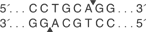
\includegraphics[scale=.5]{Sbf-I-cutsite_1_v1_000015}} }
\newglossaryentry{SbfI}{name=SbfI, description={restriction enzyme with the recognition sequence CCTGCA$\downarrow$GG} }
\newglossaryentry{XhoI}{name=XhoI, description={restriction enzyme with the recognition sequence C$\downarrow$TCGAG} }
\newglossaryentry{heterochromatin}{name=heterochromatin, description={Chromatin that remains in a highly condensed state throughout the cell cycle}}
\newglossaryentry{contig}{name=contig, description={longer consensus sequence derived from assembling smaller overlapping sequence reads}}
\newglossaryentry{linked RAD tag site}{name=linked RAD tag site, description={position in the reference sequence with at least one \gls{concordant} read pair on each side of a putative restriction site and the SE reads overlapping each other as expected from the restriction enzyme}}
\newglossaryentry{proper pair}{name=proper pair, description={read pair from illumina paired-end sequencing that got mapped to a reference in the correct orientation within a maximum expected distance from each other that is determined by the fragment size selection during the sequencing library preparation. Also called a \gls{concordant}ly mapping pair}}
\newglossaryentry{kmer}{name=kmer, description={subsequence with a specified length (k) of a longer sequence}}
\newglossaryentry{e-value}{name=Expect (E) value, description={The Expect value (E) is a parameter that describes the number of hits one can "expect" to see by chance when searching a database of a particular size}}
\newglossaryentry{read}{name=read, description={any sequence that comes out of the sequencer}}
\newglossaryentry{edit distance}{name=edit distance, description={minimum number of operations (one symbol insertion, deletion or substitution) required to change one string of symbols into another. Also known as \emph{Levenshtein distance}}}
\newglossaryentry{Ct}{name={C$_{t}$}, description={PCR cycle when a certain fluorescent threshold is reached}}
\newglossaryentry{mqs}{name={mapping quality score}, description={The mapping quality score \emph{Q} is the Phred transformation of the estimate of the probability \emph{p} that the reported mapping position does not correspond to the read's true point of origin: $Q = -10 \log_{10} p$. The way \emph{p} is estimated is different for each mapping programme, but in any case a mapping quality score \emph{Q} of 3 roughly corresponds to a mis-mapping probability \emph{p} of 0.5, i. e. the read has an estimated 50\% chance to have derived from a location other than the one reported}}
\newglossaryentry{discordant}{name=discordant, description={A read pair is called discordant if it aligns without the expected relative mate orientation (here: forward--reverse or reverse--forward) or outside the expected range of distances between mates. Note that \texttt{bowtie2} only calls discordant read pair mappings if both reads map \emph{uniquely}. Here, I am NOT adopting this requirement}}
\newglossaryentry{concordant}{name=concordant, description={A read pair is called concordant if it aligns with the expected relative mate orientation (here: forward--reverse or reverse--forward) and within the expected range of distances between mates. This is also called a \gls{proper pair}. The complement of \gls{discordant}}}
\newglossaryentry{Levenshtein distance}{name=Levenshtein distance, description={The Levenshtein distance is equal to the minimum number of operations (edits) required to transform one string into another. The allowed operations are single character insertions, deletions and substitutions. This is also known as edit distance.}}
\newglossaryentry{all pairs}{name={all pairs}, description={all the pairs of sequences below a given Levenshtein distance are identified during the graph construction phase}}
\newglossaryentry{transitive clusters}{name=transitive clusters, description={Two read clusters are merged if the distance of any pair of reads between the clusters is below threshold. After merging, the newly created cluster can contain read pairs with distance above the clustering threshold}}
\newglossaryentry{graph}{name=graph, description={A network of connected sequences. Two sequences are directly connected if they match with distance below a threshold. The distance is a measure of the strength of connection, aka "edge weight". Graphs can be stored as a list of pairs of sequences, with an optional edge weight. All graphs here should be "undirected cyclic graphs"}}
\newglossaryentry{Nmer}{name=\emph{N}mer, description={synonymous to kmer, unit, word; a subsequence of size \emph{N} that is overlapping or contiguous with the next subsequence of size \emph{N} and stored in a dictionnary (aka hash) for fast lookup}}
\newglossaryentry{population allele frequency}{name=population allele frequency, description={The population allele frequency is the (unknown) frequency of the allele in the entire population}}
\newglossaryentry{sample allele frequency}{name=sample allele frequency, description={The sample allele frequency is the frequency of the allele among the individuals in a specific sample}}
\newglossaryentry{connected component}{name=connected component, description={All nodes (here sequence reads) after all--pairs search (and before clustering!) that are directly connected by an edge or indirectly connected via several nodes belong to the same connected component} }

%----------------
% Acronyms
%----------------
\newacronym{snp}{SNP}{single nucleotide polymorphism}
\newacronym{rad}{RAD}{Restriction Site associated DNA}
\newacronym{pe}{PE}{paired-end}
\newacronym{se}{SE}{single-end}
\newacronym{bp}{bp}{base pair}
\newacronym{Mbp}{Mbp}{mega base pairs}
\newacronym{Gbp}{Gbp}{giga base pairs}
\newacronym{indel}{indel}{small sequence insertion or deletion polymorphism}
\newacronym{SAM}{SAM}{Sequence Alignment/Map format}
\newacronym{EST}{EST}{expressed sequence tag}
\newacronym{ddRAD}{ddRAD}{double digest RAD}
\newacronym{ML}{ML}{maximum likelihood}
\newacronym{SFS}{SFS}{site frequency spectrum}
\newacronym{HWE}{HWE}{Hardy Weinberg equilibrium}
\newacronym{CI}{CI}{confidence interval}
\newacronym{EM}{EM}{Expectation Maximisation}
\newacronym{DEM}{DEM}{digital elevation model}
%\usepackage[toc]{glossaries}
%\renewcommand*{\glstextformat}[1]{\textsf{#1}}
%
%\newglossaryentry{fragment}{name=fragment, description={not a PCR duplicate}}
%
%\newacronym{snp}{SNP}{single nucleotide polymorphism}

%% ******************************** SVG *************************************
%\newcommand{\executeiffilenewer}[3]{%
%	\ifnum\pdfstrcmp{\pdffilemoddate{#1}}%
%	{\pdffilemoddate{#2}}>0%
%	{\immediate\write18{#3}}\fi%
%}
%\newcommand{\includesvg}[1]{%
%	\executeiffilenewer{#1.svg}{#1.pdf}%
%	{./inkscape -z -D -f #1.svg %
%	--export-pdf=#1.pdf --export-latex}%
%	\import{./Figs/Inkscape_Graphics}{#1.pdf_tex}%
%}



%******************************** Glossary *********************************************
% *** \usepackage[toc,acronym]{glossaries}
% suppress page number list in glossary:
%\usepackage[nonumberlist]{glossaries}

%
% -- put the following code into a .latexmkrc file in the directory from where you run Latexmk --
%
%# add glossary generation to LATEXMK routine
%# ==========================================
%# taken from:
%# http://tex.stackexchange.com/questions/1226/how-to-make-latexmk-use-makeglossaries
%
%add_cus_dep('glo', 'gls', 0, 'run_makeglossaries');
%add_cus_dep('acn', 'acr', 0, 'run_makeglossaries');
%
%sub run_makeglossaries {
%  if ( $silent ) {
%    system "makeglossaries -q $_[0]";
%  }
%  else {
%    system "makeglossaries $_[0]";
%  };
%}
%
%push @generated_exts, 'glo', 'gls', 'glg';
%push @generated_exts, 'acn', 'acr', 'alg';
%$clean_ext .= ' %R.ist %R.xdy';

\makeglossaries

\renewcommand*{\glstextformat}[1]{\textsf{#1}}
%\renewcommand*{\glshyperlink}[1]{\textsf{#1}}

%--------------
% Glossary
%--------------
\newglossaryentry{fragment}{name=fragment, description={not a PCR duplicate. With paired reads from standard RAD (i. e. including random shearing of restriction fragments) typically identified by having different PE read sequences or different insert sizes after read mapping against a reference}}
\newglossaryentry{RAD tag}{name=RAD tag, description={genetic marker from RAD sequencing; the sequence up or downstream of a restriction site}}
\newglossaryentry{barcode}{name=barcode, description={short DNA sequence incorporated into adapter oligonucleotides that becomes part of the sequence read. Barcodes are used in order to be able to pool the DNA of different individuals, populations, treatments, etc. into one library that can be sequenced on one lane of an illumina flow cell}}
\newglossaryentry{index}{name=index, description={similar to barcode and serves the same purpose; generally incorporated into the centre of the adapter so that special sequencing run for the index is required} }
%\newglossaryentry{SbfI}{name=SbfI, description={restriction enzyme with the recognition sequence 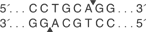
\includegraphics[scale=.5]{Sbf-I-cutsite_1_v1_000015}} }
\newglossaryentry{SbfI}{name=SbfI, description={restriction enzyme with the recognition sequence CCTGCA$\downarrow$GG} }
\newglossaryentry{XhoI}{name=XhoI, description={restriction enzyme with the recognition sequence C$\downarrow$TCGAG} }
\newglossaryentry{heterochromatin}{name=heterochromatin, description={Chromatin that remains in a highly condensed state throughout the cell cycle}}
\newglossaryentry{contig}{name=contig, description={longer consensus sequence derived from assembling smaller overlapping sequence reads}}
\newglossaryentry{linked RAD tag site}{name=linked RAD tag site, description={position in the reference sequence with at least one \gls{concordant} read pair on each side of a putative restriction site and the SE reads overlapping each other as expected from the restriction enzyme}}
\newglossaryentry{proper pair}{name=proper pair, description={read pair from illumina paired-end sequencing that got mapped to a reference in the correct orientation within a maximum expected distance from each other that is determined by the fragment size selection during the sequencing library preparation. Also called a \gls{concordant}ly mapping pair}}
\newglossaryentry{kmer}{name=kmer, description={subsequence with a specified length (k) of a longer sequence}}
\newglossaryentry{e-value}{name=Expect (E) value, description={The Expect value (E) is a parameter that describes the number of hits one can "expect" to see by chance when searching a database of a particular size}}
\newglossaryentry{read}{name=read, description={any sequence that comes out of the sequencer}}
\newglossaryentry{edit distance}{name=edit distance, description={minimum number of operations (one symbol insertion, deletion or substitution) required to change one string of symbols into another. Also known as \emph{Levenshtein distance}}}
\newglossaryentry{Ct}{name={C$_{t}$}, description={PCR cycle when a certain fluorescent threshold is reached}}
\newglossaryentry{mqs}{name={mapping quality score}, description={The mapping quality score \emph{Q} is the Phred transformation of the estimate of the probability \emph{p} that the reported mapping position does not correspond to the read's true point of origin: $Q = -10 \log_{10} p$. The way \emph{p} is estimated is different for each mapping programme, but in any case a mapping quality score \emph{Q} of 3 roughly corresponds to a mis-mapping probability \emph{p} of 0.5, i. e. the read has an estimated 50\% chance to have derived from a location other than the one reported}}
\newglossaryentry{discordant}{name=discordant, description={A read pair is called discordant if it aligns without the expected relative mate orientation (here: forward--reverse or reverse--forward) or outside the expected range of distances between mates. Note that \texttt{bowtie2} only calls discordant read pair mappings if both reads map \emph{uniquely}. Here, I am NOT adopting this requirement}}
\newglossaryentry{concordant}{name=concordant, description={A read pair is called concordant if it aligns with the expected relative mate orientation (here: forward--reverse or reverse--forward) and within the expected range of distances between mates. This is also called a \gls{proper pair}. The complement of \gls{discordant}}}
\newglossaryentry{Levenshtein distance}{name=Levenshtein distance, description={The Levenshtein distance is equal to the minimum number of operations (edits) required to transform one string into another. The allowed operations are single character insertions, deletions and substitutions. This is also known as edit distance.}}
\newglossaryentry{all pairs}{name={all pairs}, description={all the pairs of sequences below a given Levenshtein distance are identified during the graph construction phase}}
\newglossaryentry{transitive clusters}{name=transitive clusters, description={Two read clusters are merged if the distance of any pair of reads between the clusters is below threshold. After merging, the newly created cluster can contain read pairs with distance above the clustering threshold}}
\newglossaryentry{graph}{name=graph, description={A network of connected sequences. Two sequences are directly connected if they match with distance below a threshold. The distance is a measure of the strength of connection, aka "edge weight". Graphs can be stored as a list of pairs of sequences, with an optional edge weight. All graphs here should be "undirected cyclic graphs"}}
\newglossaryentry{Nmer}{name=\emph{N}mer, description={synonymous to kmer, unit, word; a subsequence of size \emph{N} that is overlapping or contiguous with the next subsequence of size \emph{N} and stored in a dictionnary (aka hash) for fast lookup}}
\newglossaryentry{population allele frequency}{name=population allele frequency, description={The population allele frequency is the (unknown) frequency of the allele in the entire population}}
\newglossaryentry{sample allele frequency}{name=sample allele frequency, description={The sample allele frequency is the frequency of the allele among the individuals in a specific sample}}
\newglossaryentry{connected component}{name=connected component, description={All nodes (here sequence reads) after all--pairs search (and before clustering!) that are directly connected by an edge or indirectly connected via several nodes belong to the same connected component} }

%----------------
% Acronyms
%----------------
\newacronym{snp}{SNP}{single nucleotide polymorphism}
\newacronym{rad}{RAD}{Restriction Site associated DNA}
\newacronym{pe}{PE}{paired-end}
\newacronym{se}{SE}{single-end}
\newacronym{bp}{bp}{base pair}
\newacronym{Mbp}{Mbp}{mega base pairs}
\newacronym{Gbp}{Gbp}{giga base pairs}
\newacronym{indel}{indel}{small sequence insertion or deletion polymorphism}
\newacronym{SAM}{SAM}{Sequence Alignment/Map format}
\newacronym{EST}{EST}{expressed sequence tag}
\newacronym{ddRAD}{ddRAD}{double digest RAD}
\newacronym{ML}{ML}{maximum likelihood}
\newacronym{SFS}{SFS}{site frequency spectrum}
\newacronym{HWE}{HWE}{Hardy Weinberg equilibrium}
\newacronym{CI}{CI}{confidence interval}
\newacronym{EM}{EM}{Expectation Maximisation}
\newacronym{DEM}{DEM}{digital elevation model}

%%%%%% -- KNITR SETUP -- %%%%%%%%%%

%************************************************************************************************
\IfFileExists{upquote.sty}{\usepackage{upquote}}{}
\begin{document}

\tableofcontents
%
%\listoffigures
%
%\listof{cmd}{List of commands}
%
%%\todototoc
\listoftodos

\printglossaries


% **************************** Define Graphics Path **************************
%% Note, every path needs to end with a "/" !!!
\ifpdf
    \graphicspath{
    {./Figs/Raster/}
    {./Figs/PDF/}
    {./Figs/}
    {../Data_analysis/reference-mapping/figure/}
    }
\else
    \graphicspath{ 
    {./Figs/Vector/}
    {./Figs/}
    {/Users/Claudius/Documents/PhD/THESIS/kks32/LaTeX/2_Chapter/Figs/Raster/}
    }
\fi

%
%
%
\chapter{Investigation into the demographic history of the hybrid zone}
%
%
%
\begin{figure}[htb]
\centering
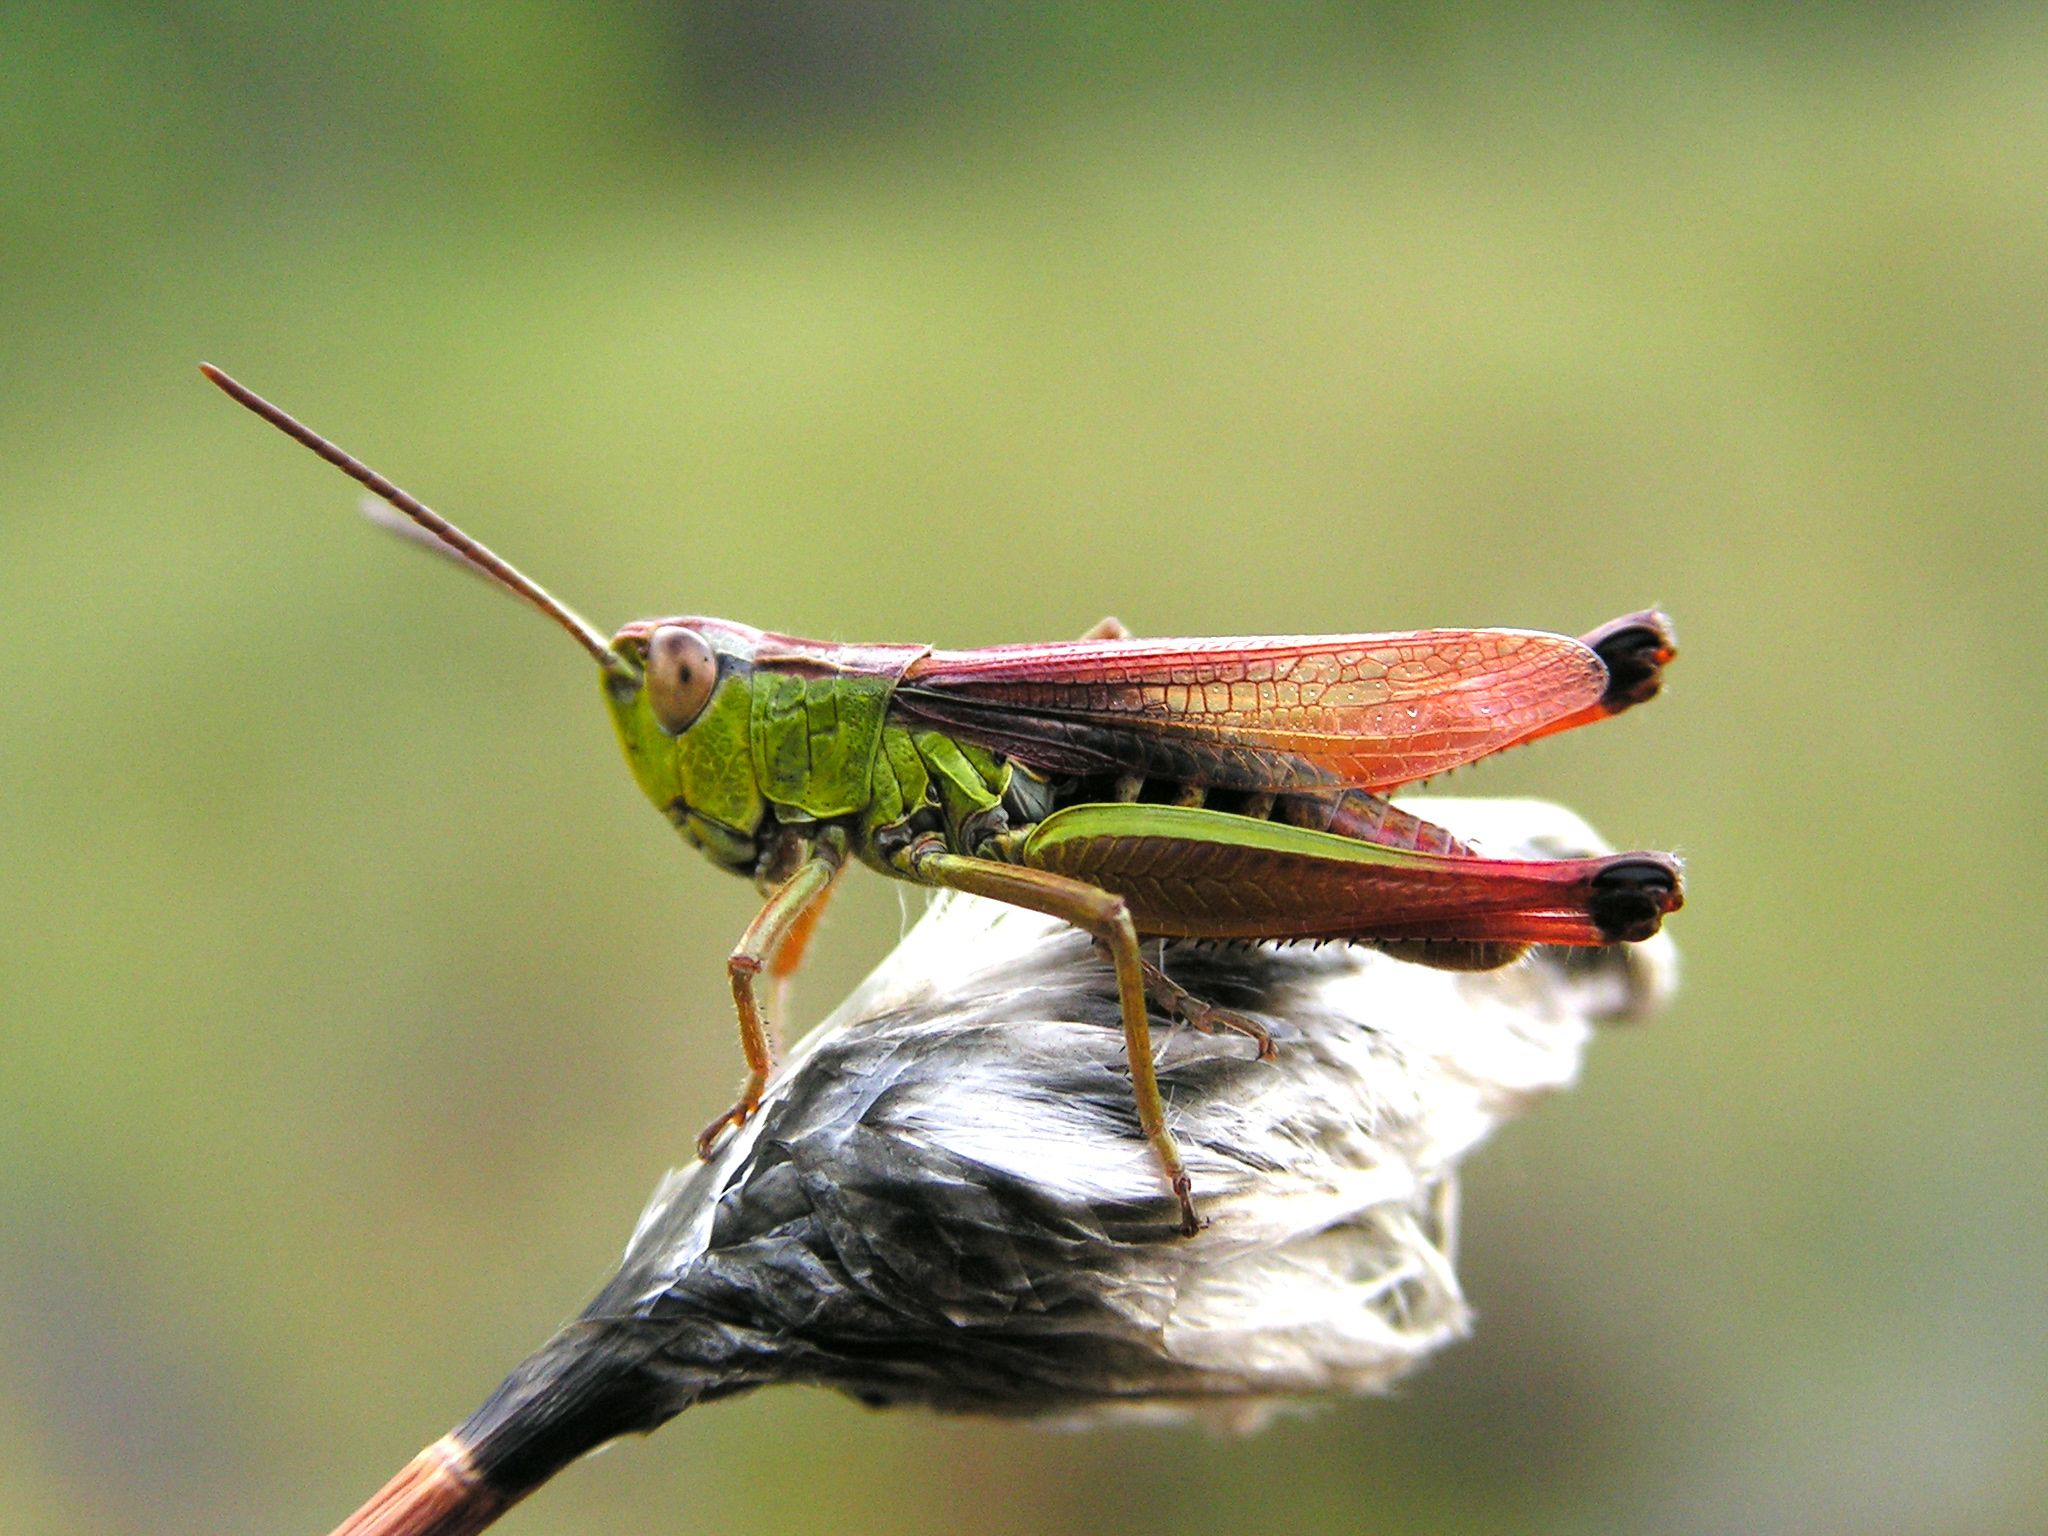
\includegraphics[width=.9\linewidth]{grasshopper}
\caption{\textit{Chorthippus parallelus parallelus}. Male individual from Finland.}
\label{Fig:grasshopper}
\end{figure}


%
%\begin{comment}
%

%\abstract{
%In this chapter I want to use all RAD data from all different libraries that I created to investigate the evolutionary history of the hybrid zone.
%
%I will first need to assemble the RAD reads of the different libraries. For that, I want to look into and test a few different programmes, pipelines and analysis protocols that have recently been published. I have created a list of 14 priority papers in my literature library in JabRef under the category \textsf{sRAD} $\rightarrow$ \textsf{RAD de novo assembly}.
%
%I will need to estimate allele frequencies from the RAD data for the two populations I got data for and use it in an ABC analysis. Parameters of interest would be:
%
%\begin{itemize}
%\item time of separation
%\item recent migration rate / rate of gene flow 
%\item recent bottlenecks
%\item signals of selection
%\end{itemize}
%
%FST: \cite{Keinan2007}, \cite{Weir2005}, \cite{McVicker2009}\\
%
%Bias: \cite{Han2014}, \cite{Andrews2016}, \cite{Gautier2012}, \cite{Luca2011}, \cite{Nielsen2011}, \cite{Crawford2012a}, \cite{Johnson2008}, \cite{Albrechtsen2010}\\
%
%2D--SFS: \cite{Gutenkunst2009}
%
%Ascertainment of SNP's in different populations. Par should have undergone recent expansion, which would have led to an increase in low frequency variants that are invariant in ERY. Fst would be close the allele frequency in PAR, i. e. low. That means ascertaining SNP's in PAR should produce a lower genome-wide Fst estimate than when ascertaining SNP's in ERY.
%
%I will need to create a list of papers to read about the technical details of ABC analysis. For the implementation, I will need the assistance of Ludovic.
%
%Finally, since I am trying to extend the scarce knowledge about the history of the hybrid zone, I will need to write a little literature review about what is known so far. Most of these papers should be there as printed copies in the hybrid zone paper box. 
%
%%\newcommand{\Todo}[1]{\todo[size=\normalsize,nolist,inline]{#1}} % don't know why \renewcommand doesn't work
%\newcommand{\Todo}[2][orange]{\todo[size=\normalsize,nolist,inline,color=#1]{#2}} % don't know why \renewcommand doesn't work
%
%\begin{itemize}
%\item RAD de novo assembly:
%	\begin{itemize}
%	\item \Todo[green]{create list of papers to read}
%	\item \Todo[green]{read through list of papers and select programmes to test}
%	\item \Todo{test selected programmes and pipelines}
%	\item \Todo{Get an estimate of the sequencing error rate from the standard RAD data.}
%	\item \Todo{run \texttt{RepeatMasker} on Radome}
%	\item \Todo{screen Radome for \textit{Wolbachia} sequences, maybe by doing a proper PE read assembly again with a proper blast annotation}
%	\item \Todo{assemble different libraries}
%	\item \Todo{estimate allele frequencies of SNP's and indels in a Bayesian framework}
%	\end{itemize}
%\item ABC:
%	\begin{itemize}
%	\item \Todo{explore \texttt{ms}}
%	\item \Todo{create list of papers to read}
%	\item \Todo{test selected programmes and pipelines}
%	\item \Todo{account for biases in the data: null alleles}	
%	\item \Todo{design ABC analysis: parameters}
%	\item \Todo{familiarise yourself with Ludovic's ABC pipeline on Iceberg}
%	\item \Todo{do ABC analysis}
%	\item \Todo{analyse posterior distributions of parameters}
%	\end{itemize}
%\item Literature review of hybrid zone history:
%	\begin{itemize}
%	\item \Todo{create list of papers to read}
%	\item \Todo{read and digest papers while writing the review}
%	\end{itemize}
%\end{itemize}
%}

%
%\end{comment}
%


\section{Introduction}

The two subspecies of the flightless grasshopper \textit{Chorthippus parallelus}, \textit{C. p. parallelus} and \textit{C. p. erythropus}, are thought to have come into secondary contact in the Pyrenees between France and Spain after the last Ice Age some 9000 years ago \citep{Hewitt1990}. They form hybrid zones across the cols of this mountain range \citep{Butlin1985,Butlin1985a}. 
Laboratory generated F$_{1}$ male hybrids between \textit{C. p. parallelus} and \textit{C. p. erythropus} from outside the hybrid zone are almost completely sterile with degenerate testes and a severely disrupted meiosis \citep{Hewitt1987}. Analysis of backcross hybrids in the laboratory suggests that a few loci of large effect contribute to hybrid sterility \citep{Llewellyn2008}. 

Males collected from the center of the hybrid zone, however, are almost completely fertile \citep{Ritchie1992}. The absence of sterile males in the center of the hybrid zone is likely due to the reconstruction of ancestral genotypes caused by selection against combinations of derived alleles in hybrids \citep{Butlin1998a}. The two subspecies are polymorphic for these negative epistatic interactions \citep{Shuker2005} and thus compatible (i.e. ancestral) alleles can reach the center of the hybrid zone. Therefore, selection is likely to restrict the introgression of those parts of the genome that are responsible for genic incompatibilities between the genomes of the two subspecies, whereas neutral loci should introgress to some extent in the two subspecies due to dispersal and recombination. 

%\cite{Butlin1998a} and \cite{Shuker2005} have shown that clines for sterility, cuticular hydrocarbons and female preference are steep in contrast to clines of several morphological characters. This indicates differential introgression across the hybrid zone. We therefore expect to find a marked increase in F$_{ST}$ in comparisons between parental populations, and steeper clines at those loci that are involved in Dobzhansky-Muller incompatibilities observed in male hybrids as compared to neutral loci.

Traditionally, population genetic analyses relied on a genotype calling step. However, with low to medium coverage (<10$\times$) next generation sequencing data there can be substantial uncertainty in genotype inferences. The major sources of error are assembly and mapping errors, base call errors and the random sampling of allele copies at hererozygous loci. If this uncertainty is ignored during downstream analyses by using the most likely genotype given the sequencing read data at a locus from an individual (and usually some hard filtering), this can lead to errors or biases in population genetic inferences \citep{Crawford2012a, Johnson2008}. Methods that avoid genotype calling by incorporating genotype uncertainty in downstream analyses can largely avoid these biases \citep{Nielsen2012, Li2011}. In addition, by avoiding SNP calling and instead incorporating uncertainty in polymorphic sites, these methods can also avoid ascertainment bias in downstream analyses \citep{Albrechtsen2010}. 

The following study is an attempt to infer some details of the demographic history of the two subspecies from patterns of genetic variation observed in next--generation sequencing data from a reduced representation library.

%
%
%
\section{Materials \& Methods}
%
%
%
%
%
\subsection{Sampling and library preparation}

Individuals from each of the two distal populations of a transect through the eastern part of the Pyrenees Mountains (Col de la Quillane) were sampled by Jamie Hutchison and Roger Butlin in 2008 and preserved in ethanol until DNA extraction in 2009. A \gls{rad} library was prepared according to the protocol of \cite{Baird2008}.\todo{add the standard RAD protocol to the appendix and refer to outline of different RAD protocols in first chapter} ~It was then sequenced on 4 lanes of an Illumina GAIIx with 51 base pair paired--end sequencing which yielded a total number of 52,872,783 read pairs.
% -- Greixer in Spain and Aunat in France -- 
%
\begin{figure}[htb]
\centering
\includegraphics[width=.9\linewidth]{map-1}
\caption{Map of sampling locations. \textsc{jh34-AU}: \textit{parallelus}; \textsc{jh30-GR}: \textit{erythropus}. \textsc{sterility centre}: marks the centre of the cline of sterility as determined by \cite{Shuker2005}. 
{\scriptsize The base map was created from two \gls{DEM} tiles  of the \href{http://www.cgiar-csi.org/data/srtm-90m-digital-elevation-database-v4-1}{SRTM 90m Digital Elevation Database v4.1} provided by CGIAR--CSI \citep{Jarvis2008}. Raster manipulations (projection, merging, clipping to polygon outline, color relief, hill shade and slope shade)  were carried out with utilities from the \href{www.gdal.org}{Geospatial Data Abstraction Library (GDAL)}. Raster overlays and map design was performed with \href{https://tilemill-project.github.io/tilemill/}{\texttt{TileMill}}, which renders maps using \href{http://mapnik.org/}{\texttt{mapnik}}. Final map image manipulations were performed with \href{https://inkscape.org/en/}{InkScape}.}
}
\label{Fig:sampling-sites-map}
\end{figure}
%

%
%
\subsection{Read filtering}
%
%
Raw sequencing reads were split by individual barcodes and filtered for base call quality with \texttt{process\_radtags} from \texttt{Stacks} \citep{Catchen2011}. Since all used barcode sequences differed from each other by at least 3 mismatches, \gls{se} reads were allowed to start with a 5 base pair sequence that differed from one of the barcodes used by 1 mismatch. Read pairs were discarded if they did not contain the remainder of the SbfI restriction site with at most one mismatch following the barcode in the \gls{se} read. Base call quality filtering was done with a sliding window across the reads. A read pair was discarded if the average Phred-scaled base call quality in a window dropped below 20. After removal of the 5 bp barcode sequence, the \gls{se} reads were 46 bp long.
%
%
\subsection{De novo assembly}
%
%
In order to create a reference sequence for the RAD tags in this library, I used an assembly strategy very similar to the one implemented in \href{https://github.com/jpuritz/dDocent}{\texttt{dDocent} }\citep{Puritz2014a}. I used all non--redundant sequence reads for de novo assembly of a RADome. I used \href{https://github.com/gui11aume/starcode}{\texttt{starcode}} (commit 1034408ca6) \citep{Zorita2015} to collapse read pairs from each individual separately into unique representatives allowing for an \gls{edit distance} of up to 2. These unique representatives are the canonical sequences from all \glspl{connected component} of the graph from an \gls{all pairs} search. Canonical sequences are chosen by highest read count, then by highest number of connections with other reads. This and the above quality filtering reduced the number of read pairs for de novo assembly to 9,179,521 (17\% of original read pair number).

After combining all \gls{se} sequences from these unique sequence pairs from all individuals into one fasta file, I have used \href{https://github.com/torognes/vsearch}{\texttt{Vsearch}} (commit 1116d6167b) \citep{Rognes2016} with its subcommand \texttt{cluster\_fast} for heuristic clustering with a pairwise identity threshold of 0.8 of a query sequence with the centroid of a growing cluster. Identity is defined as 1 minus \gls{edit distance}, but excluding terminal gaps. Thus an indel between two reads will only contribute once towards their edit distance.

Next, I have used the \texttt{uclust} format output of \texttt{Vsearch} together with the collapsed sequences from \texttt{starcode} to create a clustering output in the format of the output from \href{https://sourceforge.net/projects/bio-rainbow/files/}{\texttt{rainbow cluster} }\citep{Chong2012}. I then ran \texttt{rainbow div} on this cluster file. This programme recursively splits the initial clusters into putative alleles/haplotypes while keeping track of the relationships between split clusters in a tree--like data structure. These split clusters are next merged back recursively along this tree structure with \texttt{rainbow merge} that uses the similarity between \gls{pe} reads to determine whether two split clusters should be merged. Remember that the standard RAD protocol \citep{Baird2008} includes random shearing of restriction fragments. This produces \gls{pe} reads of variable distances from the same RAD tag \citep{Etter2011}. The unique feature of \texttt{rainbow} is to be able to utilise these shotgun--type \gls{pe} reads to distinguish alleles from paralogs. In addition, after recursively merging split clusters into putative RAD loci, \texttt{rainbow merge} also performs a local de novo assembly with the sequences of each merged cluster using \gls{se} and \gls{pe} reads. From the assembly output I then extracted the \gls{se} RAD tag sequences together with their longest \gls{pe} read contig (separating each with a sequence of 10 N's) using \texttt{gawk} code from \texttt{dDocent}. 

Finally, since the merge process of \texttt{rainbow} depends on overlap between \gls{pe} reads from the same RAD locus, it could be incomplete when coverage is low. I therefore clustered the \texttt{rainbow} contigs again with the \texttt{Vsearch} subprogramme \texttt{cluster\_fast}, this time with an identity threshold of 0.9 and producing a majority consensus sequence from a multiple alignment of the sequences in each cluster of \texttt{rainbow} contigs.

The assembled RADome contains 583,312 contigs and a total length of 97 \gls{Mbp}. In the following I will frequently refer to it as the Big Data reference assembly. 
%
%
\subsection{Read mapping}
%
%
I mapped all quality filtered reads against the Big Data reference with the programme \href{http://bowtie-bio.sourceforge.net/bowtie2/manual.shtml}{\texttt{bowtie2}} \citep{Langmead2012}. I ran \texttt{bowtie2} in end--to--end mode, i. e. without soft--clipping of query sequences. Further, I specified "very--sensitive" search mode with a seed length of 20. I allowed gaps to be up to 10 bp long, but I disallowed gaps within 4 bp of either end of the read. In addition I specified a high penalty of 10 for alignments against ambiguous characters in the reference. In each reference contig, \gls{se} RAD tag and \gls{pe} contig were separated by 10 N's. This high penalty therefore makes successful read alignments across the gap between \gls{se} RAD tag and \gls{pe} read contig very unlikely. Further, I specified a minimum fragment length of 60 for \gls{proper pair} read alignments, thus allowing some overlap between reads in a pair. 

Note that previous analysis of the same read data had revealed a high proportion of PCR duplicates. Although standard RAD data from paired--end sequencing allows the detection and removal of PCR duplicates, I have opted not to do so for convenience. The following analyses all depend on the correct estimation of genotype likelihoods which assumes that reads are sampled independently from the true genotype. The following analyses should therefore be repeated excluding reads from PCR duplicates. Although variance and uncertainty in parameter estimates will then increase as a result of lower coverage, I do not expect the global estimates to change much, i. e. those which are based on data from $>$1 million nucleotide sites.

%
%
\subsection{Filtering}
%
%

There are 4,575 contigs with \gls{se} reads that map to the \gls{pe} part of the contig, i. e. which do not pass the \textit{mismapping} filter. I have also filtered \glspl{contig} for excessive coverage by \gls{se} reads, which map to the \gls{RAD tag} part of each contig (i. e. next to the restriction site). The coverage by \gls{pe} reads is much more dependent on the length of the contig. With this filter a contig has excessive coverage if in any of the individual BAM files it has \gls{se} read coverage above the 99th percentile of the individual's coverage distribution. I have thus excluded 2,282 contigs due to excessive coverage. Since many false--positive \glspl{snp} fall within low--complexity sequences \citep{Li2014}, I have detected those regions within the \emph{Big Data} reference assembly with \texttt{dustmasker} \citep{Morgulis2006} and excluded them from further analysis. The above filters have excluded 10\% of the reference from further analysis, leaving 88 \gls{Mbp}. %before filtering: sum of interval length from Big_Data_ref.fa.bed, after filtering: sum of interval length from Big_Data_Contigs.noSEgt2.nogtQ99Cov.noDUST.bed
I then went on to extract those bits of the filtered reference that have sufficient data for downstream analyses. I used the \texttt{samtools depth} command to get the read count for all positions and for all 36 individuals across the filtered reference. I then extracted those positions where at least 15 individuals have each at least 3$\times$ coverage. I only counted reads with a mapping quality greater than 5. This reduces the number of sites to 2\% of the original \emph{Big Data} reference assembly or 2 \gls{Mbp}, spread over 34,967 contigs. The first 6 base pairs of each contig are the remainder of the SbfI restriction site (\texttt{TGCAGG}) and therefore not variable. I have excluded those sites as well from further analysis. In addition to the excessive coverage filter, I have also applied a HWE filter to the remaining sites in order to reduce false heterozygotes caused by reads from paralogous sequences mapping to the same position in the reference. I have used the programme \texttt{ANGSD} \citep{Korneliussen2014} to estimate per site inbreeding coefficients ($F_{site}$) as well as LRT p--values using genotype likelihoods \citep{Vieira2013}. I removed entire contigs that had a site with a negative estimate of inbreeding coefficient and a p--value for deviation of $F_{site}$ from 0 of less than 0.05.  I estimated inbreeding coefficients for each population separately as well as for both populations taken together. The latter increased sample size for the estimation of $F_{site}$ but also increased estimates of $F_{site}$ for \glspl{snp} with different allele frequencies in the two populations. This filter removed 217 contigs. This has left 1,799,962 filtered sites on 34,750 contigs for further analysis. Inspection of the global, i. e. across sample, coverage distribution revealed that there were 12,693 sites with total coverage greater than 1000$\times$. I have therefore also determined the 99th percentile of the global per--site coverage distribution and removed all contigs with a position that had coverage greater than the global 99th percentile. This has removed 69,438 sites on 407 contigs leaving 
1,730,524 sites on 34,343 contigs for further analysis.
%
\begin{figure}[htb]
\centering
\begin{knitrout}
\definecolor{shadecolor}{rgb}{0.969, 0.969, 0.969}\color{fgcolor}

{\centering \includegraphics[width=.9\linewidth]{figure/global-coverage-dist-1} 

}



\end{knitrout}
\caption{Global distribution of coverage with reads of mapping quality greater than 5 over 1.7 million sites in the \emph{Big Data} reference after filtering.}
\label{Fig:global-coverage-dist}
\end{figure}
%
The average per site, per individual coverage across the 1.7M filtered sites is 6.3$\times$ (fig. \ref{Fig:global-coverage-dist}).
%
\begin{figure}[htb]
\centering
\begin{knitrout}
\definecolor{shadecolor}{rgb}{0.969, 0.969, 0.969}\color{fgcolor}

{\centering \includegraphics[width=.9\linewidth]{figure/ind-cov-dist-1} 

}



\end{knitrout}
\caption{Individual coverage distributions from reads with mapping quality greater than 5 over 1.7 million sites in the \emph{Big Data} reference after filtering. red: \textit{erythropus}, green: \textit{parallelus}.}
\label{Fig:individual-coverage-dist}
\end{figure}
%

%
%
\subsection{PCA}
%
%
I have used \texttt{ANGSD}  \citep{Korneliussen2014} to estimate posterior genotype probabilities across all sites using as prior a \gls{ML} estimate of the minor \gls{population allele frequency} per site across all individuals and the assumption of \gls{HWE} \citep{Kim2011}. Although the assumption of \gls{HWE} may well be violated, it should only make genotype probability estimates more similar between divergent individuals. Therefore, any major divergence detected between individuals based on these genotype probabilities cannot be an artifact of this prior. At low coverage, the identification of the minor allele can be uncertain. The estimation of the minor allele frequency incorporated this uncertainty \cite[suppl. mat.]{Skotte2012}. I have then estimated the \gls{ML} global unfolded \gls{SFS} based on per--site \gls{sample allele frequency} likelihoods, again across all individuals, using \texttt{ANGSD} \citep{Nielsen2012, Korneliussen2013}. This global \gls{SFS} then served as prior to estimate per--site \gls{sample allele frequency} posterior probabilities. Thus for each site $2N+1$ probabilities were calculated. Finally, I estimated a covariance matrix with \texttt{ngsCovar} \citep{Fumagalli2014} between all 36 individuals by summing over genotype probabilities and weighting each site by its probability of being variable \citep[eq. 19 and 20]{Fumagalli2013}. I then performed an eigen--decomposition on the resulting covariance matrix with the \texttt{R} function \texttt{prcomp}.
%
%
\subsection{$F_{ST}$}
%
%
Using \texttt{ANGSD} and its subprogramme \texttt{realSFS} \citep{Korneliussen2014}, I have determined a ML estimate of the global \emph{unfolded} 2D--\gls{SFS} that contains the joint sample allele frequencies of the non--reference allele from \textit{erythropus} and \textit{parallelus}. I required a nucleotide site to have sequence reads from at least 9 individuals in each population. The 2D--SFS contains the joint frequencies from approximately 1.13 million sites. This global unfolded 2D--\gls{SFS} was then used as (empirical) prior for posterior sample allele frequency probabilities from which the posterior expectation of $F_{ST}$ per site is calculated using \texttt{realSFS} from ANGSD \citep{Fumagalli2013}. This programme reports the numerator and denominator for either Reynolds' \citep[eq. 3]{Fumagalli2013} or Hudson/Bhatia's $F_{ST}$ \citep[eq. 9 and 10]{Bhatia2013} for each site. I am not reporting estimates of $F_{ST}$ per site due to their large variance \citep{Weir2005}. Instead I am reporting \emph{average} $F_{ST}$ across sites within a contig or the global average $F_{ST}$ across all sites. This average is always calculated by summing nominator and denominator across sites and then taking the ratio \citep{Bhatia2013}.
In order to investigate the dependence of $F_{ST}$ on SNP ascertainment in one or the other population, I have calculated ML estimates of population minor allele frequencies with \texttt{ANGSD} \citep{Kim2011}. I have then used these allele frequencies to subset sites into minor allele frequency classes and estimated average $F_{ST}$ for each bin as before.
%
%
\subsection{Genetic diversity estimates}
%
%
I have calculated ML estimates of the \emph{folded} global \gls{SFS}, i. e. including all sites across contigs, for \textit{erythropus} and \textit{parallelus} separately with \texttt{ANGSD} and its subprogramme \texttt{realSFS} \citep{Korneliussen2014}. 
I required 9 individuals to have read data in order to include a site into the estimation. Since I noticed a considerable amount of variability in the ML estimates of SFS from repeated runs of the programme \texttt{realSFS}, I turned off its accelerated \gls{EM} algorithm, extended the maximum number of \gls{EM} iterations to 50,000 and specified a \textit{tolerance} of 1e-06, which is the minimum difference in likelihood between two successive \gls{EM} iterations and therefore a stopping criterium. These modifications completely removed the variability in SFS estimates, but also greatly extended running time, particularly for the \gls{SFS} of \textit{parallelus}. The programme \texttt{realSFS} allows bootstrapping the \gls{SFS}, i. e. re--estimation of \gls{SFS} from nucleotide sites resampled with replacement.~\comment{The CI estimated from these bootstraps will be too narrow, since it ignores that sites in the same contig are not independent and the SFS estimated is therefore a \emph{composite likelihood} estimate.} I derived the global estimates of the number of segregating sites and the average number of pairwise differences from the global folded \gls{SFS} according to equations 1.3 and 1.4 in \cite{Wakeley2009}. The estimates of global Tajima's D are based on these estimates and equation 2.17 in \cite{Gillespie2004}.\todo{include those equations verbatim here} ~The estimates for \textit{parallelus} are based on 1,214,939 sites, the estimates for \textit{erythropus} are based on 1,638,468 sites. I have also estimated Tajima's D per--contig with the empirical Bayes method described in \cite{Korneliussen2014}. This uses the ML estimate of the global folded \gls{SFS} as prior for posterior sample allele frequency probabilities that are then summed across the sites in each contig to get the per--contig estimate of \gls{SFS}.

%
%
%
\section{Results \& Discussion}
%
%
%

%
%
\subsection{Genetic differention between \textit{erythropus} and \textit{parallelus}}
%
%
Figure \ref{Fig:PCA} shows a principal component analysis of genotypic covariances between all 36 individuals of \textit{erythropus} and \textit{parallelus} taking SNP and genotype uncertainty into account. Almost 1/4 of the total genotypic variance is explained by the first principal component which clearly separates the two subspecies. The second component captures only 3\% of the total genotypic variance. This confirms estimates of genetic differentiation by \cite{Cooper1995} based on sequence variation at a single nuclear locus that the two subspecies are genetically distinct. Individual \texttt{par\_34-1} seems to be considerably less differentiated from \textit{erythropus} than the other \textit{parallelus} individuals. This may be due to insufficient information because of extremely low coverage (see fig. \ref{Fig:individual-coverage-dist})
%
\begin{figure}[htb!]
\centering
\begin{knitrout}
\definecolor{shadecolor}{rgb}{0.969, 0.969, 0.969}\color{fgcolor}

{\centering \includegraphics[width=.9\linewidth]{figure/PCA-1} 

}



\end{knitrout}
\caption{Principal component analysis with genotype probabilities across 1.7 million sites from all 36 individuals of \textit{erythropus} and \textit{parallelus}. Each site was weighted by its probability of being variable during the estimation of genotypic covariances between individuals.}
\label{Fig:PCA}
\end{figure}
%

I estimated posterior expectations of $F_{ST}$ from 1.6 million sites across 32,706 contigs. Note, that this included 0.5 million sites for which there were fewer than 9 individuals with read data in one of the two populations.
%
\begin{figure}[htb]
\centering
\begin{knitrout}
\definecolor{shadecolor}{rgb}{0.969, 0.969, 0.969}\color{fgcolor}

{\centering 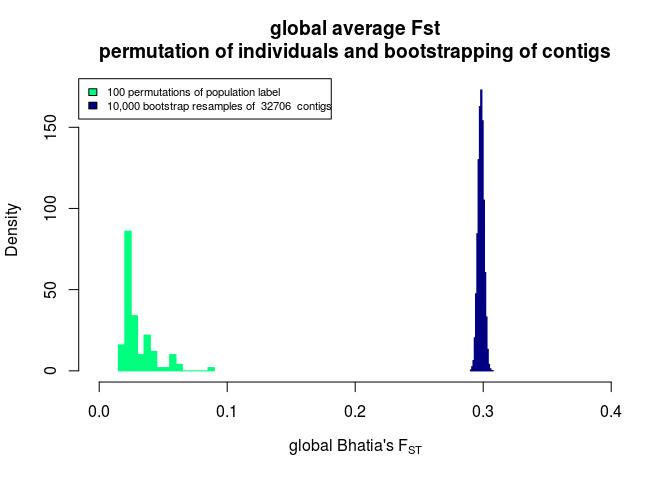
\includegraphics[width=.9\linewidth]{figure/permut-global-fst-hist-1} 

}



\end{knitrout}
\caption{Resampling based estimation of the variance of global $F_{ST}$ (blue) and distribution of global $F_{ST}$ when randomly permuting individuals into two populations (green).}
\label{Fig:global-fst}
\end{figure}
%
The global average Hudson/Bhatia's estimate of $F_{ST}$ is 0.298 with a bootstrap 95\% \gls{CI} between 0.294 and 0.303 (see fig. \ref{Fig:global-fst}). Note, that the 95\% \gls{CI} only captures the variance due to sampling loci in the genome (\emph{genetic sampling} according to \cite{Weir1996}, p. 161), not the variance due to sampling individuals from the population. The latter could be estimated by bootstrapping individuals from each population. Estimating \gls{CI}'s by bootstrapping over contigs assumes that they are independent replicates of the evolutionary process in the history of the two subspecies, i. e. that they are unlinked. However, with the standard RAD protocol \citep{Baird2008}, two RAD tags (here called contigs) are recovered from each restriction site. The bootstrap \gls{CI} for genome-wide $F_{ST}$ computed here may therefore slightly underestimate uncertainty. Also note that the null distribution of global $F_{ST}$, estimated by randomly permuting individuals into two populations, does not include 0. There therefore seems to be a positive bias in the estimation of global $F_{ST}$ of about 0.0249.

Figure \ref{Fig:fst-by-ascert-class} shows the dependence of average $F_{ST}$ on the minor allele frequency when only sites are included that are polymorphic in the ascertainment population. Not surprisingly, SNP ascertainment in one of the two populations lowers average $F_{ST}$ estimates since it also excludes highly differentiated sites where the ascertainment sample is fixed for one allele.
%
\begin{figure}[htb]
\centering
\begin{knitrout}
\definecolor{shadecolor}{rgb}{0.969, 0.969, 0.969}\color{fgcolor}

{\centering \includegraphics[width=.9\linewidth]{figure/fst-by-ascertainment-class-1} 

}



\end{knitrout}
\caption{$F_{ST}$ by ascertainment class. The global average $F_{ST}$ when using all sites, i. e. without SNP ascertainment, is shown as a grey line.}
\label{Fig:fst-by-ascert-class}
\end{figure}
%
When ascertaining SNP sites in \textit{erythropus} or \textit{parallelus}, in each case the average $F_{ST}$ estimate tends to decrease with decreasing minor allele frequency. This is consistent with both populations having undergone a recent population expansion where rare alleles are more likely to be private to one population. This is made evident by the estimate of global unfolded 2D-\gls{SFS} that was used as prior for per--site $F_{ST}$ estimates (fig. \ref{Fig:unfolded-2D-SFS}). Since these sites have a low allele frequency differentiation, they lower the average $F_{ST}$ estimate. In contrast, if one or both populations had undergone a recent population bottleneck, variable sites would more often be ancient and polymorphic in the ancestral population. Sites with rare alleles in the bottlenecked population would therefore also include those that have drifted apart in allele frequency between the two populations, thus increasing average $F_{ST}$ estimates \citep{Bhatia2013}.
%
\begin{figure}[H]
\centering
\begin{knitrout}
\definecolor{shadecolor}{rgb}{0.969, 0.969, 0.969}\color{fgcolor}

{\centering \includegraphics[width=.9\linewidth]{figure/unfolded-2D-SFS-1} 

}



\end{knitrout}
\caption{ML estimate of the joint sample allele frequencies of the non--reference allele for \textit{parallelus} (PAR) and \textit{erythropus} (ERY). The joint frequency class (0,0) has been set to zero for the purpose of better visualisation.}
\label{Fig:unfolded-2D-SFS}
\end{figure}
%

A ML estimate of the number of nucleotide sites with fixed differences between these two samples of 18 individuals each of \textit{erythropus} and \textit{parallelus} can also be extracted from the unfolded 2D--\gls{SFS}: 418 or 0.69\% of polymorphic sites. \cite{Whitlock2015} have recently described a method to detect loci likely under spatially heterogeneous selection by modelling the neutral distribution of $F_{ST}$ for specific demographic scenarios. Figure \ref{Fig:fst-by-contig-hist} shows the observed distribution of $F_{ST}$ across all contigs. The method of \cite{Whitlock2015} could be applied to this distribution for inference of likely demographic scenarios.

%
\begin{figure}[htb]
\centering
\begin{knitrout}
\definecolor{shadecolor}{rgb}{0.969, 0.969, 0.969}\color{fgcolor}

{\centering \includegraphics[width=.9\linewidth]{figure/fst-by-contig-hist-1} 

}



\end{knitrout}
\caption{Distribution of $F_{ST}$ across contigs.}
\label{Fig:fst-by-contig-hist}
\end{figure}
%
\clearpage
%
%
\subsection{Genetic diversity within \textit{erythropus} and \textit{parallelus}}
%
%
Figure \ref{Fig:folded-sfs} shows the ML estimate of global folded \gls{SFS} for \textit{erythropus} and \textit{parallelus}. The conspicuous spike in frequency for the minor allele count of 2 in \textit{parallelus} is not compatible with any demographic scenario. Bootstrapping contigs instead of nucleotide sites could show whether this is an artifact due to one or a few contigs. However, even when disregarding frequency class 2, the folded \gls{SFS} of \textit{parallelus} seems to be more right--skewed, that is having a greater proportion of low--frequency variants than \textit{erythropus}. 
%
\begin{figure}[htb]
\centering
\begin{knitrout}
\definecolor{shadecolor}{rgb}{0.969, 0.969, 0.969}\color{fgcolor}

{\centering \includegraphics[width=.9\linewidth]{figure/folded-sfs-1} 

}



\end{knitrout}
\caption{ML estimate of the global minor allele frequency spectrum for \textit{erythropus} and \textit{parallelus}. The \gls{SFS} of  \textit{erythropus} is based on 1.6 million, the one of \textit{parallelus} on 1.2 million nucleotide sites.}
\label{Fig:folded-sfs}
\end{figure}
%
Note, that this \gls{SFS} is not based on called \glspl{snp}. Instead it is based on per--site sample allele frequency likelihoods that incorporate the genotype uncertainty of each individual due to binomial sampling of alleles as well as sequencing and read alignment error \citep{Li2008, Li2011, Nielsen2012}. It does not therefore suffer from the ascertainment bias observed in previous studies that were based on sites detected as polymorphic in a specific sample \citep{Albrechtsen2010, Korneliussen2013}. This ascertainment bias has led to a relative excess of intermediate versus low frequency classes. 

The \gls{SFS} has however not yet been corrected for bias due to allele--drop--out \citep{Luca2011, Cariou2016}. Allele--drop--out is a problem that has affected previous types of genetic markers like microsatellites or AFLP's, usually known under the term "null alleles". \cite{Arnold2013} and \cite{Gautier2012} have shown with simulations that loci affected by allele--drop--out show a greater proportion of intermediate allele frequencies as compared to loci not affected. They therefore show a relative excess of observed nucleotide expected heterozygosity ($\pi_{Tajima}$). My data filtering, that included filtering for minimum coverage and for minimum number of individuals with read data, should have enriched for sites less affected by allele--drop--out. Those sites show the opposite bias towards a relative excess of low--frequency variants \citep{Arnold2013}. Since the same filtering thresholds were applied to the data from \textit{erythropus} and \textit{parallelus} and since the \textit{parallelus} sample has generally much lower coverage (see fig. \ref{Fig:individual-coverage-dist}), it seems plausible that the sites used to estimate the \gls{SFS} for \textit{parallelus} have been relatively more enriched for those less affected by allele--drop--out. This may explain the relative excess of low--frequency variants in \textit{parallelus} compared to \textit{erythropus}. Filtering with different minimum--individual or coverage thresholds could shed some light on the effect of allele--drop--out on the global folded \gls{SFS}. 

The allele--drop--out problem is a missing data problem and to some extent similar to the missing data problem caused by low coverage next--generation sequencing. Both increase false homozygote calls for true heterozygotes and both therefore lead to a deviation of observed genotype frequencies from \gls{HWE}. The algorithms implemented in \texttt{ANGSD} and described in \cite{Li2011} and \cite{Nielsen2012} are designed to deal with this problem by
\begin{enumerate}
\item incorporating genotype uncertainty into downstream population genetic analyses
\item "imputing" genotype likelihoods by estimating the population minor allele frequency using the raw genotype likelihoods from all individuals in the same population and \emph{assuming \gls{HWE}}.
\end{enumerate}
I therefore expect \texttt{ANGSD} to reduce the effects of allele--drop--out on population genetic analyses.
%
\begin{figure}[htbp]
\centering
\begin{knitrout}
\definecolor{shadecolor}{rgb}{0.969, 0.969, 0.969}\color{fgcolor}

{\centering \includegraphics[width=.75\linewidth]{figure/folded-sfs-boot-exh-ery-1} 

}



\end{knitrout}
\begin{knitrout}
\definecolor{shadecolor}{rgb}{0.969, 0.969, 0.969}\color{fgcolor}

{\centering \includegraphics[width=.75\linewidth]{figure/folded-sfs-boot-exh-par-1} 

}



\end{knitrout}
\caption{Estimation of the variance of the global folded \gls{SFS} by bootstrap resampling of nucleotide sites.}
\label{Fig:folded-sfs-boot-exh}
\end{figure}
%
\\
Figure \ref{Fig:folded-sfs-boot-exh} shows that despite the large amount of sites included in the ML estimation, there is still considerable uncertainty in the global folded \gls{SFS}, particularly for \textit{parallelus}. This could be explained by the lower average sequence coverage for individuals from the \textit{parallelus} population (see fig. \ref{Fig:individual-coverage-dist}).
%
\begin{figure}[htb]
\centering
\begin{knitrout}
\definecolor{shadecolor}{rgb}{0.969, 0.969, 0.969}\color{fgcolor}

{\centering \includegraphics[width=.75\linewidth]{figure/S-and-Pi-1} 
\includegraphics[width=.75\linewidth]{figure/S-and-Pi-2} 

}



\end{knitrout}
\caption{Global estimates of the proportion of segregating sites and average number of pairwise differences per nucleotide site derived from ML estimates of the global folded \gls{SFS}. The distributions are based on 200 bootstrap resamples of sites.}
\label{Fig:S-and-Pi}
\end{figure}
%
\\
The number of segregating sites ($S$) and the average number of pairwise differences ($\pi_{Tajima}$) are summary statistics of the \gls{SFS}. While $S$ weights each site equally, intermediate frequency variants contribute much more to the magnitude of $\pi$ than high-- and low--frequency variants \cite[eq. 1.4]{Wakeley2009}. Figure \ref{Fig:S-and-Pi} shows both estimates for \textit{erythropus} and \textit{parallelus} together with distributions from 200 bootstrap resamples of nucleotide sites. Both diversity estimates are significantly higher in \textit{parallelus} than in \textit{erythropus}. This seems at odds with the expectation from the hitherto proposed demographic model of a postglacial expansion of \textit{C. p. parallelus} towards central and western Europe from a glacial refuge in the Balkans \citep{Cooper1995, Lunt1998}. \textit{C. p. erythropus} in the Pyrenees on the other hand is expected to be derived from several smaller refuges in southern Spain, i. e. its expansion after the last Ice Age would have covered a much smaller distance. According to this model one would expect the \textit{parallelus} subspecies to have undergone a long series of founder events which should have reduced genetic diversity much more so than for the \textit{erythropus} subspecies \citep{Luca2011}. That ancestral \textit{parallelus} and \textit{erythropus} expanded from their glacial refuges as a "wave", i. e. without colonisation by rare long--distance migration, is made unlikely by at least two observations: 
\begin{itemize}
\item the colonisation of Britain by \textit{C. p. parallelus} before the flooding of the English Channel after the last Ice Age \citep{Cooper1995},
\item the clines for several markers in the Pyrenean hybrid zone between the two subspecies that are too wide to be explained by the dispersal rate of this species of 30 m/generation \citep{Nichols1994}. 
\end{itemize}
The higher genetic diversity in Pyrenean \textit{parallelus} is not unique to this study though. So reported \cite{Lunt1998} intraregional $K_{S}$ values of a mitochondrial sequence variation that were 1.5 times higher in Pyrenean \textit{parallelus} than in Pyrenean \textit{erythropus} and \cite{Llewellyn2008}, table 3--3, found that nucleotide diversity ($\pi_{Tajima}$) was higher in \textit{parallelus} than in \textit{erythropus} from the Pyrenees in 5 out of 7 expressed sequences.
%
\begin{figure}[htb]
\centering
\begin{knitrout}
\definecolor{shadecolor}{rgb}{0.969, 0.969, 0.969}\color{fgcolor}

{\centering \includegraphics[width=.75\linewidth]{figure/Tajimas-D-1} 

}



\end{knitrout}
\begin{knitrout}
\definecolor{shadecolor}{rgb}{0.969, 0.969, 0.969}\color{fgcolor}

{\centering \includegraphics[width=.75\linewidth]{figure/Tajimas-D-by-contig-1} 

}



\end{knitrout}
\caption{Top: ML estimate of global Tajima's D and distribution of Tajima's D from 200 bootstraps of the global folded \gls{SFS}. Bottom: Distribution of Tajima's D estimates for each contig.}
\label{Fig:Tajimas-D}
\end{figure}
%
\\
The Tajima's D estimates also differ significantly between the two subspecies (fig. \ref{Fig:Tajimas-D}). While the value for \textit{erythropus} is slightly positive (0.0561), the value for \textit{parallelus} is clearly negative (\ensuremath{-0.614}). The latter would be consistent with a recent increase in population size. However -- as already explained above for the apparent right--skew of the global folded \gls{SFS} of \textit{parallelus} -- this difference in Tajima's D might also be caused at least in part by the greater enrichment of sites that are not affected by allele--drop--out in \textit{parallelus} versus \textit{erythropus} due to lower coverage and applying the same filtering thresholds. Again, investigating the effect of varying filtering thresholds for the \textit{parallelus} sample on the Tajima's D estimate could already show whether the difference in Tajima's D is indeed caused by differences in sequence coverage between the two subspecies. Interestingly, despite a slightly positive global Tajima's D, the distribution of Tajima's D per contig has a strong peak below zero in \textit{erythropus} (fig. \ref{Fig:Tajimas-D}). 
%%
%\begin{figure}[htb]
%\centering
%<< Tajimas-D-by-contig, out.width='.65\\linewidth', echo=FALSE, cache=TRUE, warning=FALSE>>=
%@
%\caption{Distribution of Tajima's D estimates for each contig.}
%\label{Fig:Tajimas-D-by-contig}
%\end{figure}
%%



%----------------------------
% Bibliography
%----------------------------

\bibliographystyle{elsarticle-harv}
\bibliography{/Users/Claudius/Documents/MyLiterature/Literature}
%
\end{document}

